\documentclass[a4paper,12pt,french]{article}
\usepackage[margin=2cm]{geometry}
\usepackage[thinfonts,latinmath]{uglix2}
\nouveaustyle


\pagestyle{empty}
\begin{document}
	\titre{Devoir en temps libre 1}{\premiere}{pour le 16/09}

\exo{}\\
Soit $\lambda$ un nombre réel.\\
A, B et C sont trois points tels que $\quad AB=20\lambda +12$, $\quad BC=15(\lambda+1)\quad$ et $\quad AC=25\lambda +19$.\\
On considère le point D tel que ABCD est un parallélogramme.
\begin{enumerate}[\bfseries 1.]
	\item 	Faire un schéma et rappeler une condition nécessaire et suffisante pour qu'un parallélogramme soit un rectangle.
	\item 	Déterminer toutes les valeurs de $\lambda$ pour lesquelles ABCD est un rectangle.
	\item	 Quelle est alors la longueur BD ?\\
\end{enumerate}




\exo{}
\begin{enumerate}[\bfseries 1.]
	\item 	Rappeler la définition d'une fonction affine.
	\item 	Démontrer la proposition suivante :\\
			\og Si $f$ est une fonction affine, alors pour tous réels $u$ et $v$, $\quad f\left(\dfrac{u+v}{2}\right)=\dfrac{f(u)+f(v)}{2}$ \fg.
	\item	Compléter la phrase suivante qui permet de reformuler cette propriété en terme de moyenne :\\
	Si $f$ est une fonction affine, alors l'image par $f$ de la moyenne de deux nombres réels est égale à \dotfill\\
\end{enumerate}


\exo{}
On considère un entier naturel $n$ non nul.\\
On pose $\quad S_n=1+2+3+...+(n-2)+(n-1)+n$.
\begin{enumerate}[\bfseries 1.]
	\item 	En remarquant que $\quad S_n=n+(n-1)+(n-2)+...+3+2+1,\quad$ déterminer une expression de $2S_n$ en fonction de $n$.
	\item 	En déduire une expression de $S_n$ en fonction de $n$.
	\item	Calculer $\quad 1+2+3+...+2021$.
\end{enumerate}
\begin{encadrecolore}{Un peu d'histoire}{UGLiBlue}
\begin{minipage}{12cm}
	Selon une légende, pendant un cours, l'instituteur de \textbf{Carl Friedrich Gauss} (mathématicien allemand, 1777-1855) voulant obtenir le calme dans sa classe, demanda à ses élèves de calculer la somme 1 + 2 + 3 + ... + 100.\\
	C'est en utilisant la technique précédente que Carl Friedrich trouva rapidement la réponse.
\end{minipage}
\begin{minipage}{4cm}
	\flushright
	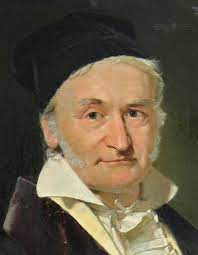
\includegraphics[width=3cm]{Gauss}\\
\end{minipage}
	




\end{encadrecolore}
\end{document}
